\chapter{Progettazione}
\label{capitolo5}
\thispagestyle{empty}

\noindent Nei paragrafi successivi sono illustrate le fasi di implementazione del gestore di dati personali, motivando le scelte implementative e le eventuali differenze che si sono verificate rispetto a quanto detto in Analisi.

Per la realizzazione del gestore \`e stato utilizzato il linguaggio Java\cite{javalanguagespecs} \cite{java8api}.

Fra i principi generali seguiti in Progettazione troviamo l’inversione delle dipendenze, la separazione delle responsabilit\`a, il principio di sostituibilit\`a di Liskov e il gi\`a citato rasoio di Occam. Secondo il principio di inversione delle dipendenze, \`e necessario che le dipendenze presenti all’interno del codice non siano fra classi ma fra interfacce, in modo da evitare che la struttura possa risentire di cambiamenti che avvengono a basso livello. Il principio di separazione delle responsabilit\`a stabilisce che a ogni classe \`e attribuito un solo compito, da svolgere e completare interamente, ma mai pi\`u di uno: lo sviluppo di classi aventi pi\`u responsabilit\`a genera dipendenze non volute fra le classi, rendendo il codice fragile. Il principio di sostituibilit\`a di Liskov, infine, si applica ai casi di ereditariet\`a fra classi e ne regola il rapporto: ogni sottoclasse deve poter essere utilizzata al posto della classe base senza che sia evidenziata la differenza.

\section{Flusso del programma}
inserire grafico

\section{Accounting}
\label{sec:P-accounting}
\begin{figure} [h]
	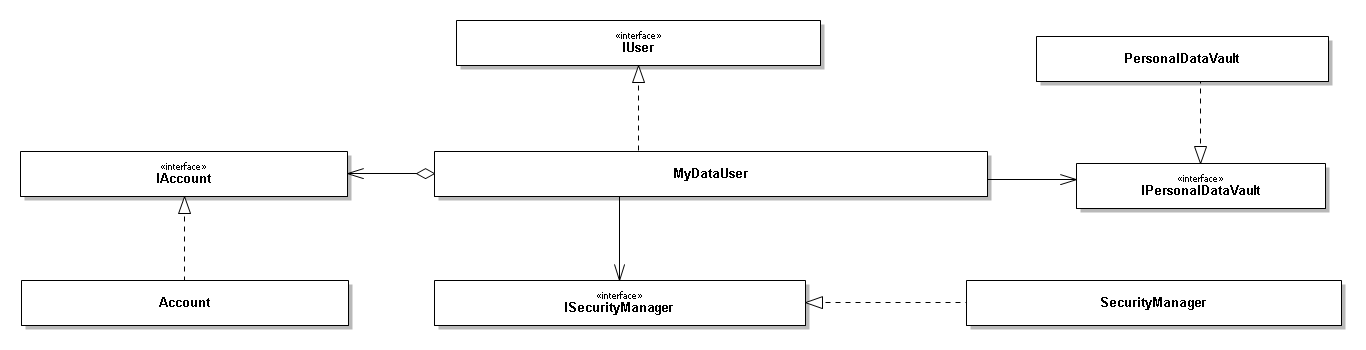
\includegraphics[width=\linewidth]{pictures/Accounting-closed.png}
	\caption{Diagramma UML delle classi di gestione degli account}
	\label{fig:Accounting-closed}
\end{figure}
Osservando il diagramma UML in figura \ref{fig:Accounting-closed} si osserva al centro la classe corrispondente all’utente \textit{MyData} che, confermando quanto detto in Analisi, \`e collegata agli account dei servizi e al \texttt{PersonalDataVault} dell’utente. Una novit\`a \`e invece rappresentata dalla coppia \texttt{ISecurityManager}, \texttt{SecurityManager} creata per soddisfare i requisiti di sicurezza relativi alla mutua autenticazione fra utente e servizio. Si \`e deciso di sviluppare separatamente questa classe per un principio di separazione delle responsabilit\`a e per consentire una estendibilit\`a pi\`u semplice in caso di sviluppi futuri.

\subsection{IUser, MyDataUser}
\begin{figure} [h]
	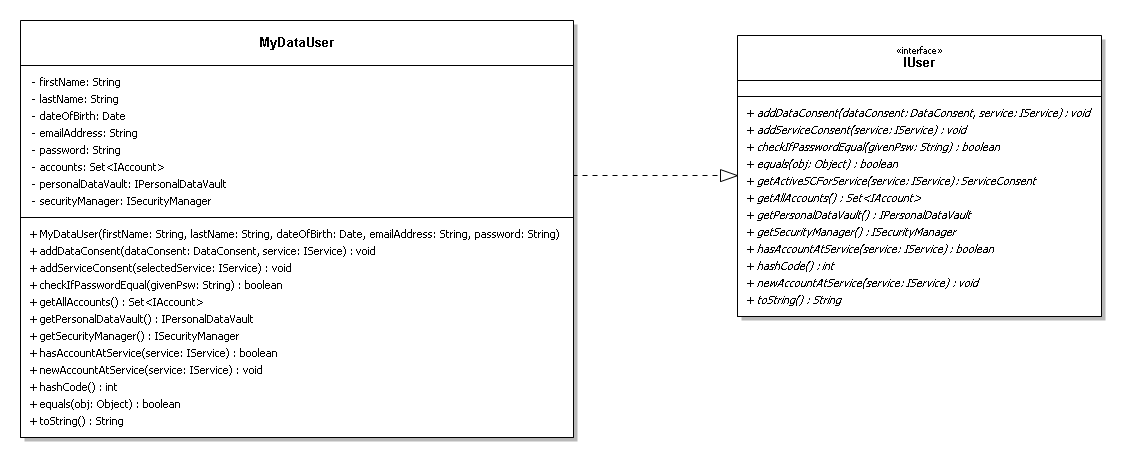
\includegraphics[width=\linewidth]{pictures/Accounting-MyDataUsr.png}
	\caption{Diagramma UML dell'implementazione di un account MyData}
	\label{fig:Accounting-MyDatUsr}
\end{figure}
Questa classe modella un generico utente dell’architettura \textit{MyData}. I field al suo interno sono un esempio delle caratteristiche che si \`e scelto di modellare e fra essi i pi\`u rilevanti sono indirizzo email e password in quanto permettono il login per utenti gi\`a registrati. L’indirizzo mail \`e stato adottato, inoltre, come identificatore unico di un utente all’interno di \textit{MyData} e questa caratteristica \`e stata implementata mediante l’override della funzione \texttt{equals(Object obj)}.

Si evidenzia inoltre la presenza di un \texttt{Set<IAccount> accounts} che realizza l’associazione fra un utente e gli account presso i servizi a cui si \`e registrato. La scelta di un \texttt{Set} permette di implementare il vincolo secondo cui ogni utente pu\`o avere un solo account presso un certo servizio ed \`e efficace anche perch\'e \`e superfluo mantenere un insieme ordinato di account.

Questa classe, inoltre, ha la funzione di interfacciare gli altri componenti del gestore, compresa la GUI, con gli account utente. A tal fine presenta i metodi \texttt{addServiceConsent (IService service)}, \texttt{addDataConsent (DataConsent dataConsent, IService service)}, \texttt{hasAccountAtService (IService service)}.  La classe \texttt{Account}, infatti, \`e stata modellata con visibilit\`a package protected per impedire l’accesso a classi esterne al package \texttt{users}: di conseguenza, anche la creazione di nuovi account avviene attraverso questa classe, in particolare nella funzione \texttt{newAccountAtService (IService service)}. All’interno del metodo troviamo l’istanziazione di un nuovo account insieme ad una chiamata alla classe \texttt{ConsentManager} che realizza quanto anticipato al paragrafo \ref{subsec:A-Consent} a pagina \pageref{subsec:A-Consent}. In questo modo si ottiene un esempio di \textit{Service Linking} e l’esito di questa operazione viene concretizzato in un oggetto \texttt{ServiceConsent}. Si rimandano per\`o ulteriori dettagli a quanto evidenziato nella sezione \ref{sec:P-AutorizzazioniEConsent} a pagina \pageref{sec:P-AutorizzazioniEConsent}.

\subsection{IAccount, Account}
\label{subsec:P-Account}
\begin{figure} [h]
	\centering
	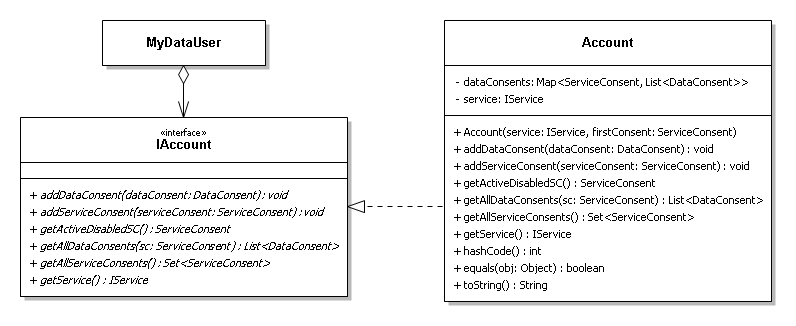
\includegraphics[width=0.95\linewidth]{pictures/Accounting-Account.png}
	\caption{Diagramma UML dell'implementazione di un account presso un servizio}
	\label{fig:Accounting-Account}
\end{figure}
La classe \texttt{Account} \`e abbastanza semplice poich\'e si occupa semplicemente di implementare la logica di basso livello nelle operazioni di gestione degli account.

Fra queste vi sono i controlli sullo stato dei Consent memorizzati, la gestione dello storico di tutti i Consent emessi per quel servizio \texttt{service} o ancora il matching fra i due tipi di Consent (\texttt{ServiceConsent}, \texttt{DataConsent}, dettagliati al paragrafo \ref{subsec:P-ServiceConsentDataConsent} a pagina \pageref{subsec:P-ServiceConsentDataConsent}).

La memorizzazione dei Consent all’interno della classe \`e stata ottenuta mediante l’utilizzo combinato delle strutture dati \texttt{Map<ServiceConsent, \-List\-<Data\-Consent>{}>}. Questa modalit\`a permette di esprimere diversi concetti a livello semantico. Innanzitutto per i Consent sul flusso di dati si \`e scelto di utilizzare la classe base \texttt{DataConsent} invece che le sue due implementazioni, in modo da poterli memorizzare indiscriminatamente. Ci\`o verifica l’utilizzo del principio di sostituibilit\`a di Liskov. Inoltre, la scelta di una \texttt{List} come value all’interno di una mappa permette di descrivere un flusso di dati (all’interno dello stesso \texttt{ServiceConsent}) per il quale si sono rivelate necessare una molteplicit\`a di interazioni fra \textit{Source} e \textit{Sink}, ognuna delle quali modellata da un \texttt{DataConsent}.

Ad ogni istanza di \texttt{ServiceConsent} corrisponde quindi una \texttt{Collection} dei \texttt{DataConsent} emessi durante il periodo di validit\`a dello stesso ed \`e possibile avere un unico \texttt{ServiceConsent} attivo in un determinato istante di tempo.

\section{Servizi}
\label{sec:P-Service}
\begin{figure} [h]
	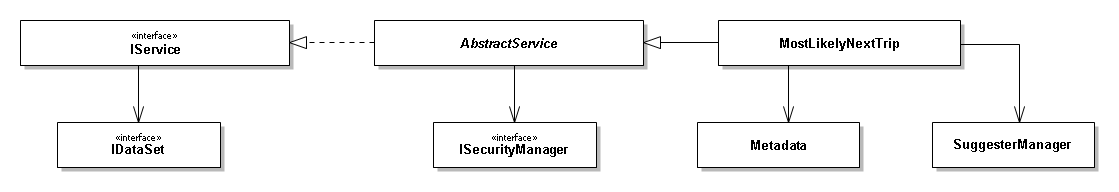
\includegraphics[width=\linewidth]{pictures/Services-closed.png}
	\caption{Diagramma UML per la rappresentazione di un servizio e delle sue dipendenze}
	\label{fig:Services-closed}
\end{figure}
Il diagramma UML in figura \ref{fig:Services-closed} mostra l’implementazione proposta per l’utilizzo di servizi all’interno dell’architettura \textit{MyData}. L’interfaccia \texttt{IService} e la classe astratta \texttt{AbstractService} sono state realizzate al fine di mediare l’interazione fra servizio concreto (in questo caso \textit{Most Likely Next Trip}) e Operatore (ad esempio, classi \texttt{ServiceRegistry} o \texttt{IMyData}). In questo senso, si pu\`o dire che la classe \texttt{AbstractService} raccoglie a fattore comune le operazioni comuni a tutti i servizi, lasciando alle classi figlie il compito di realizzare solo le parti fortemente dipendenti dalla particolare business logic. Per realizzare un nuovo servizio \`e necessario quindi creare una classe che estende \texttt{AbstractService}: nel caso di studio, essa \`e la classe \texttt{MostLikelyNextTrip}, che si interfaccia con il servizio di calcolo del prossimo viaggio pi\`u probabile \cite{MLNT} \texttt{SuggesterManager}.

\subsection{IService, AbstractService, MostLikelyNextTrip}
\begin{figure} [h]
	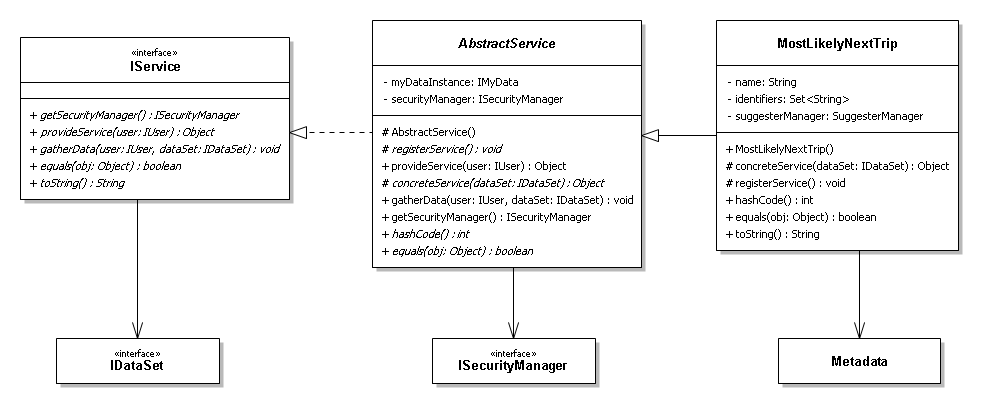
\includegraphics[width=\linewidth]{pictures/Services-open.png}
	\caption{Diagramma UML dell'implementazione di un servizio generico}
	\label{fig:Services-open}
\end{figure}
Il livello pi\`u astratto di definizione dei servizi in \textit{MyData} \`e rappresentato dall’interfaccia \texttt{IService}, e permette il loro riferimento all’interno dell’architettura. Fra i metodi esposti si evidenziano \texttt{provideService (IUser user)} e \texttt{gatherData (IUser user, dataSet IDataSet)}, che costituiscono i punti di ingresso e di uscita del flusso di dati utilizzati e prodotti dal servizio.

L’interfaccia viene implementata parzialmente dalla classe \texttt{AbstractService}. 

Il metodo \texttt{provideService} raccoglie a fattore comune la richiesta di un \texttt{OutputDataConsent} al \texttt{ConsentManager}, seguita dall’effettiva richiesta di dati inoltrata al \texttt{PersonalDataVault} tramite una richiesta alla classe \texttt{MyData}. Infine, viene restituito il risultato della chiamata alla funzione \texttt{abstract protected concreteService (IDataSet dataSet)}: la visibilit\`a garantisce che dall’esterno venga chiamato solo il metodo esposto dall’interfaccia \texttt{IService}. La signature astratta obbliga la ridefinizione del metodo nella classe figlia, che conterr\`a l'effettiva \textit{business logic} del servizio.

Il metodo \texttt{gatherData} segue la stessa sequenza di passi: la richiesta al \texttt{ConsentManager} di un \texttt{InputDataConsent} e l’interazione con il \texttt{PersonalDataVault} mediante Operatore \textit{MyData} sono per\`o preceduti da alcuni controlli sui dati in ingresso, al fine di verificare la legittimit\`a della richiesta.

Fra i metodi astratti si evidenzia infine \texttt{registerService()}, da invocare all’interno del costruttore della classe figlia. Durante la chiamata a procedura, il servizio concreto specifica quali tipi di dato utilizzer\`a mediante l’utilizzo delle costanti descritte in dettaglio nella sezione \ref{subsec:P-metadata}.

Della classe implementativa \texttt{MostLikelyNextTrip} si evidenzia solo la presenza dello stato interno, dove sono contenuti il nome, identificatore unico del servizio, e il \texttt{Set<String>} che contiene i tipi di dato utilizzati dal servizio.

\section{Operatore MyData}
Come previsto in fase di Analisi (sezione \ref{sec:A-mydataop}), si \`e proceduto alla realizzazione dell'Operatore \textit{MyData} tramite separazione delle responsabilit\`a, ottenendo come risultato le classi presentate nelle sottosezioni seguenti.

La sottosezione \ref{subsec:P-imydataMyData} presenta il nodo centrale del gestore di dati personali, che si occupa del coordinamento fra servizi, utente e Personal Data Storage. Svolge, insieme al \texttt{ConsentManager} (realizzato nella sottosezione \ref{subsec:P-CMConsStatus}), la funzione di \textit{policy enforcement}.

La sottosezione \ref{subsec:P-SecMan} presenta il componente \texttt{SecurityManager}, esempio di gestore delle politiche di sicurezza all'interno del progetto.

Infine, la sottosezione \ref{subsec:P-serviceregistry} presenta l'implementazione del \textit{Service Registry}.

\subsection{IMyData, MyData}
\label{subsec:P-imydataMyData}
\begin{figure} [h]
	\centering
	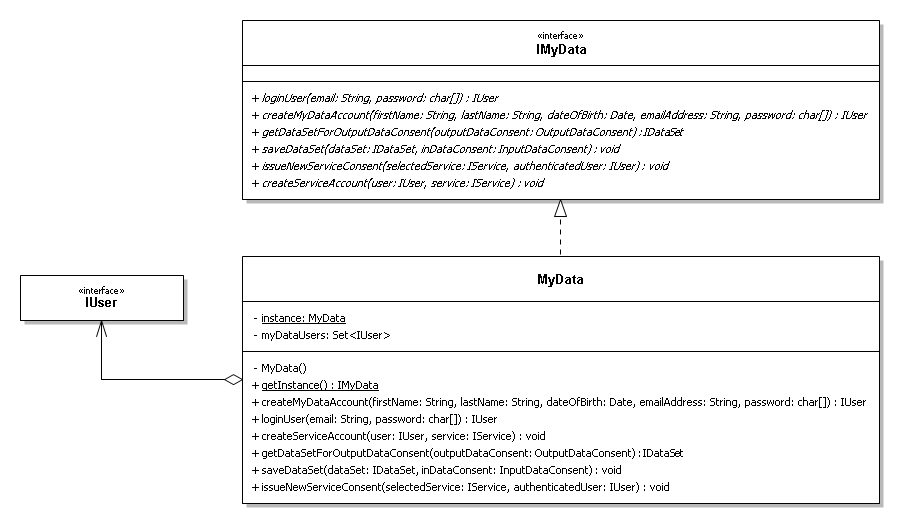
\includegraphics[width=0.8\linewidth]{pictures/MyData.png}
	\caption{Diagramma UML dell'implementazione di parte dell'Operatore MyData}
	\label{fig:Accounting-MyData}
\end{figure}
La classe \texttt{MyData} svolge all’interno del gestore di dati personali un importante ruolo di coordinamento fra le parti poich\'e realizza al suo interno una parte dell’Operatore \textit{MyData}, secondo quanto specificato in \ref{sec:A-mydataop}. Essa \`e il punto di riferimento per l’interfaccia utente a cui fornisce i dati da elaborare e mostrare a video e dalla quale riceve le richieste effettuate dall’utente.

Innanzitutto, si occupa di registrare e autenticare gli utenti (metodi \texttt{createMyDataAccount} e \texttt{loginUser}) in modo da impedire la creazione di duplicati. I controlli in questo senso vengono effettuati su un \texttt{HashSet<IUser>} contenuto all’interno della classe (si sfrutta la propriet\`a della struttura dati \texttt{Set} di non ammettere duplicati). La creazione di un nuovo account presso un determinato servizio viene gestita da questa classe tramite invocazione dell’opportuno metodo esposto dall’interfaccia \texttt{IUser}, insieme alla richiesta di nuovi \texttt{ServiceConsent} in caso di utente gi\`a registrato.

In secondo luogo, ogni servizio che ha richiesto e ottenuto il permesso di accedere a uno specifico insieme di dati personali di un utente fa riferimento alla classe \texttt{MyData}, che si occupa di intercedere presso il Personal Data Vault per ottenere quanto richiesto. L’operazione si svolge sia per i dati in ingresso che per i dati in uscita dal Vault mediante i metodi \texttt{getDataSetForOutputDataConsent (OutputDataConsent outputDataConsent)} e \texttt{saveDataSet (IDataSet dataSet, InputDataConsent inDataConsent)}. In entrambi i casi, viene controllata la validit\`a del Consent emesso prima di effettuare la richiesta di dati personali.

Infine, si evidenzia la realizzazione della classe \texttt{MyData} come Singleton mediante l’utilizzo di un costruttore privato e di un campo \texttt{instance} di tipo \texttt{MyData}. Ci\`o assicura la presenza di un unico Operatore di questo tipo all’interno del programma.

\subsection{SecurityManager}
\label{subsec:P-SecMan}
\begin{figure} [h]
	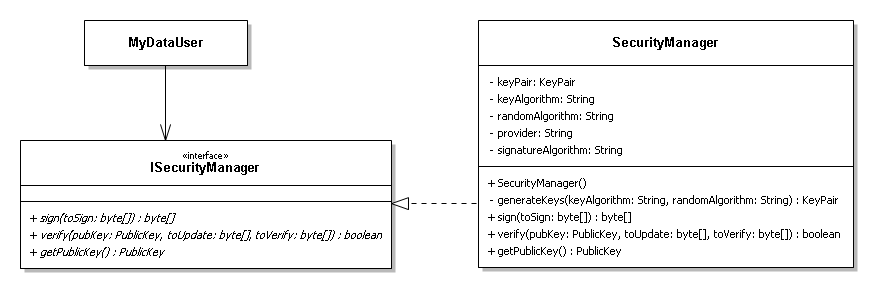
\includegraphics[width=\linewidth]{pictures/Accounting-SecurityManager.png}
	\caption{Diagramma UML del gestore delle operazioni di sicurezza}
	\label{fig:Accounting-SecurityManager}
\end{figure}
Come anticipato nella sezione \ref{sec:P-accounting}, si \`e resa necessaria l'implementazione di una entit\`a che garantisse il rispetto di alcune politiche di sicurezza.

In particolare, in questa implementazione si \`e scelto di dare maggiore rilevanza all'aspetto di reciproca autenticazione fra utente e servizio, piuttosto che ad altre problematiche quali ad esempio memorizzazione e trasmissione sicura dei dati. A tal fine si \`e scelto di utilizzare alcuni componenti gi\`a pronti all'interno dell'infrastruttura Java, in particolare all'interno della Java Cryptography Architecture \cite{javacrypto}.

Per realizzare un protocollo di sfida e risposta, la classe \texttt{SecurityManager} contiene una coppia di chiavi \texttt{KeyPair}, insieme ad alcune costanti che rappresentano gli algoritmi ed il provider scelto per l'implementazione degli stessi.

L'interfaccia \texttt{ISecurityManager} ha la funzione di astrarre dalla particolare implementazione (ogni servizio potrebbe ad esempio preferire una implementazione specifica), e pertanto espone solamente i metodi di firma e verifica necessari al completamento dell'operazione di autenticazione.

\subsection{ServiceRegistry}
\label{subsec:P-serviceregistry}
\begin{figure} [h]
	\centering
	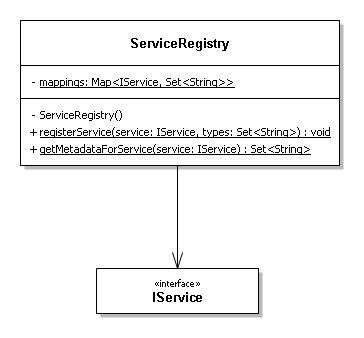
\includegraphics[width=0.5\linewidth]{pictures/ServiceRegistry.png}
	\caption{Diagramma UML dell'implementazione del Service Registry}
	\label{fig:ServiceRegistry}
\end{figure}
Ogni servizio che voglia essere utilizzabile all’interno dell’infrastruttura \textit{MyData} deve, per prima cosa, registrarsi all’interno del \textit{Service Registry}. In fase di registrazione, ogni servizio dichiara inoltre i tipi di dato necessari per il suo funzionamento, al fine di agevolare gli scambi di dati con altre entit\`a dell’infrastruttura, siano esse \textit{Source} o \textit{Sink}.

Per questo motivo, la classe \texttt{ServiceRegistry} ha come responsabilit\`a fondamentale quella di mantenere al suo interno le corrispondenze fra i servizi registrati e i tipi di dato: ci\`o viene realizzato mediante l’utilizzo di una \texttt{Map<IService, Set<String>{}>}.

Come per la classe \texttt{ConsentManager} (analizzata pi\`u in dettaglio nella sottosezione \ref{subsec:P-CMConsStatus}), anche in questo caso ho cercato di rendere il \textit{Service Registry} il pi\`u possibile indipendente tramite l’uso di metodi statici e la scelta di un costruttore privato. I metodi \texttt{registerService(IService service, Set<String> types)} e \texttt{Set<String> getMetadataForService(IService service)} incapsulano quelli di basso livello esposti dalla struttura dati \texttt{Map}, aggiungendo gli opportuni controlli sui parametri in ingresso. In particolare, \`e possibile registrare un servizio mediante la procedura \texttt{registerService}, e ottenere i tipi di dato registrati mediante la funzione \texttt{getMetadataForService}.

\section{Autorizzazioni e Consent}
\label{sec:P-AutorizzazioniEConsent}
\begin{figure} [h]
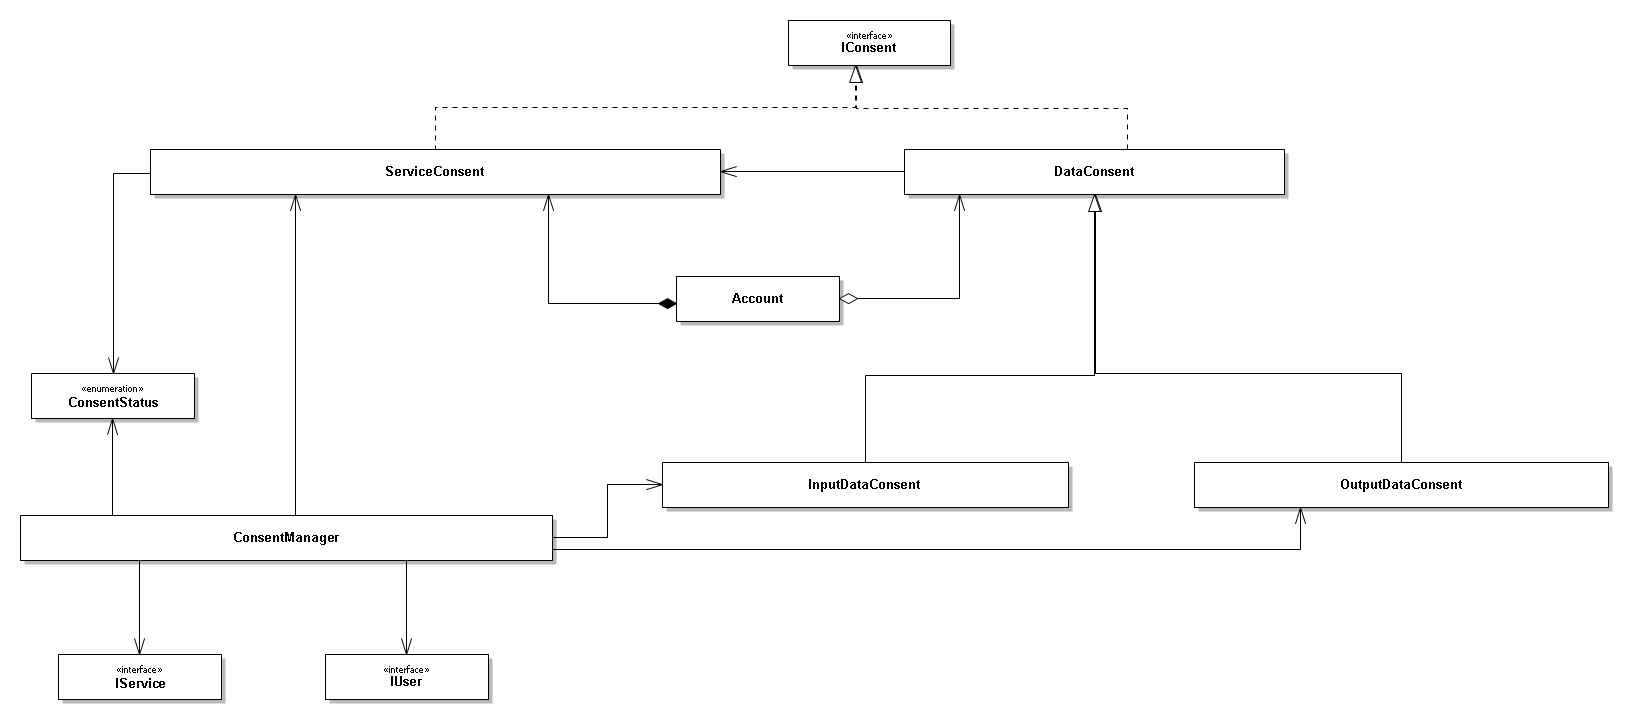
\includegraphics[width=\linewidth]{pictures/Auth-closed.png}
\caption{Diagramma UML dell'architettura per la gestione dei permessi}
\label{fig:Auth-closed}
\end{figure}
All'interno dell'architettura realizzata per la gestione delle autorizzazioni e dei permessi \`e possibile individuare alcune entit\`a fondamentali: la classe \texttt{ConsentManager}, che realizza il gestore di permessi previsto nella sezione \ref{sec:A-mydataop}, e le due tipologie di permessi, anch’esse previste in fase di Analisi (sottosezione \ref{subsec:A-Consent}).

\`E presente infine anche l’enumerativo \texttt{ConsentStatus}, attraverso il quale si rappresentano gli stati del rapporto fra un utente ed un servizio generici.

\subsection{ConsentManager, ConsentStatus}
\label{subsec:P-CMConsStatus}
\begin{figure} [h]
	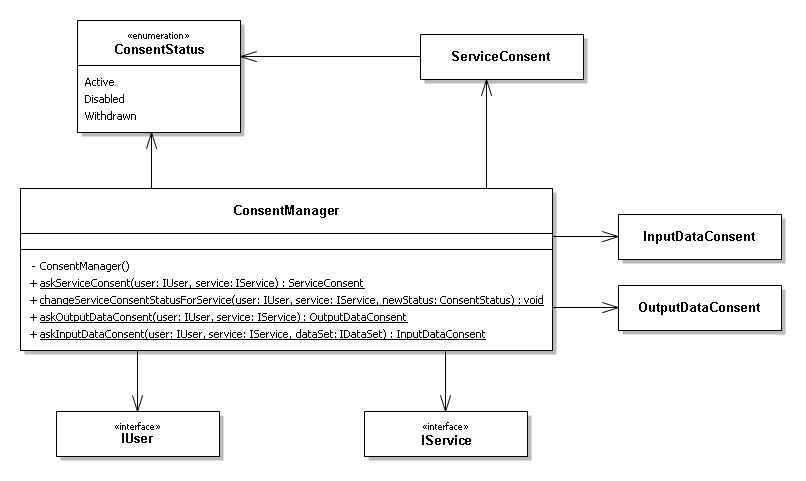
\includegraphics[width=\linewidth]{pictures/Auth-CM.png}
	\caption{Diagramma UML del gestore di permessi}
	\label{fig:Auth-CM}
\end{figure}
La classe \texttt{ConsentManager} si occupa dell’erogazione, in caso di richiesta legittima, di vari tipi di permessi ai servizi che ne fanno richiesta. Poich\'e il suo scopo \`e quello di garantire il rispetto di un determinato protocollo di assegnazione dei permessi, essa \`e innanzitutto una classe implementativa e per questo motivo non \`e previsto alcun tipo di astrazione (ad esempio tramite interfaccia).

Si potrebbe considerare di rendere la classe \texttt{final}, per impedire estensioni o ridefinizioni del comportamento. Le motivazioni a supporto di questa scelta risiedono nella garanzia di una maggiore sicurezza. Tuttavia, nel complesso, ci\`o porterebbe ad una eccessiva rigidit\`a del codice, impedendo aggiornamenti del protocollo anche in casi di legittima necessit\`a.

Per la sua implementazione, ho cercato di fare in modo che essa realizzasse un servizio il pi\`u possibile indipendente dal resto dell’architettura circostante. Pertanto, la classe \texttt{ConsentManager} non mantiene alcuno stato interno, presenta costruttore privato e non ha dipendenze rilevanti. Inoltre, poich\'e la procedura di verifica dei requisiti \`e costante e indipendente dai parametri di ingresso, ogni metodo \`e stato realizzato come \texttt{static}. 

I tipi di Consent erogati dalla classe \texttt{ConsentManager} sono \texttt{ServiceConsent}, \texttt{InputDataConsent} e \texttt{OutputDataConsent}, ognuno con un metodo dedicato. \`E presente anche la procedura \texttt{changeServiceConsentStatusForService (IUser user, IService service, ConsentStatus newStatus)}, che permette all’utente di cambiare lo stato del \texttt{ServiceConsent} correntemente attivo o disabilitato, secondo quanto previsto dalle specifiche di \textit{MyData} e successivamente in fase di Analisi (sottosezione \ref{subsec:A-Consent}).

\subsection{ServiceConsent, DataConsent}
\label{subsec:P-ServiceConsentDataConsent}
\begin{figure} [h]
	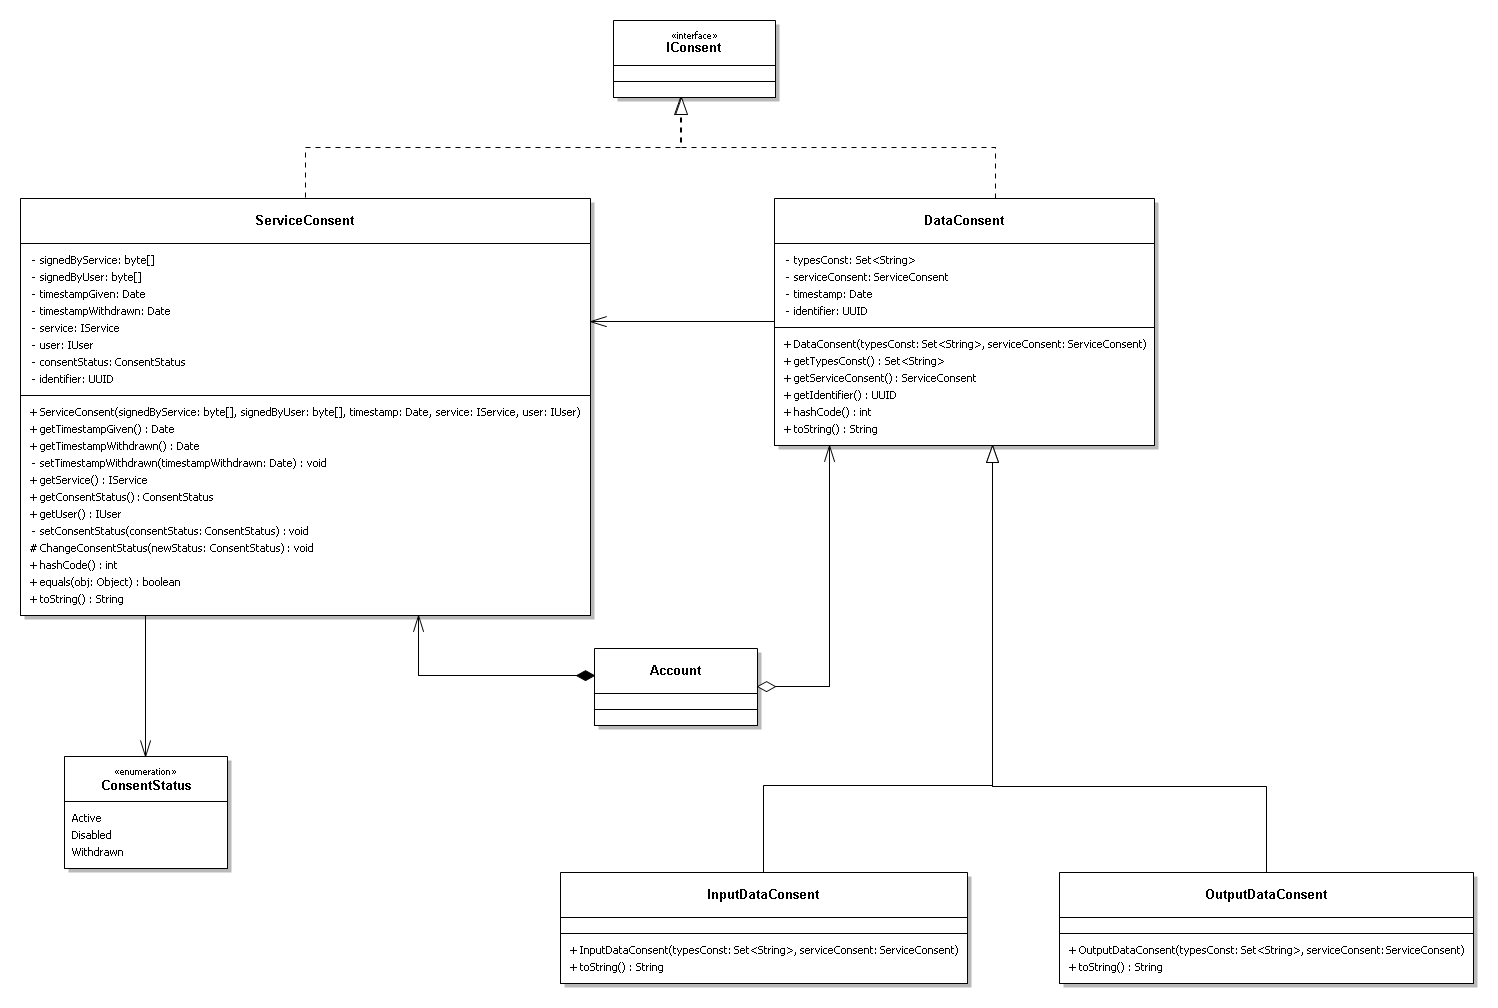
\includegraphics[width=\linewidth]{pictures/Auth-Consents.png}
	\caption{Diagramma UML dei due tipi di permessi e delle loro dipendenze}
	\label{fig:Auth-Consents}
\end{figure}
I permessi utilizzati all’interno del gestore di dati personali ed erogati dalla classe \texttt{ConsentManager} sono istanze delle classi \texttt{ServiceConsent}, \texttt{InputDataConsent} e \texttt{OutputDataConsent}. Come \`e possibile osservare dal diagramma UML in figura \ref{fig:Auth-Consents}, \texttt{InputDataConsent} e \texttt{OutputDataConsent} estendono la classe \texttt{DataConsent}: la loro funzione \`e principalmente semantica, in quanto non aggiungono logica al programma ma descrivono il verso del flusso di dati che si crea con il Personal Data Vault. Pertanto, descriver\`o principalmente le caratteristiche delle classi \texttt{ServiceConsent} e \texttt{DataConsent}, che costituiscono il punto focale della realizzazione dei permessi descritti in \textit{MyData}.

Nonostante la differenza di realizzazione e di utilizzo, entrambe le classi \texttt{ServiceConsent} e \texttt{DataConsent} implementano una interfaccia comune \texttt{IConsent}. Questa \`e una interfaccia \textit{marker} necessaria per esprimere una somiglianza a livello semantico, in quanto entrambe le classi descrivono un tipo di autorizzazione.

Dal diagramma UML \`e possibile dedurre il ruolo della classe \texttt{Account} rispetto ai due tipi di Consent. Come accennato infatti in \ref{subsec:P-Account}, essa mantiene al suo interno una mappa di corrispondenze fra \texttt{ServiceConsent} e liste di \texttt{DataConsent}.

Nel primo caso, la relazione \`e rappresentata mediante il simbolo “rombo nero”, che qualifica la classe \texttt{Account} come “contenitore” di istanze della classe \texttt{ServiceConsent}. In particolare, il rombo nero descrive un tipo di relazione molto stretta fra le due parti, e la scelta \`e dovuta alle specifiche di \textit{MyData}, secondo cui non \`e possibile registrarsi presso un servizio senza ottenere un Consent. Ci\`o \`e stato implementato mediante l’emissione di un \texttt{ServiceConsent} prima della creazione effettiva dell’account, e il legame fra i due avviene tramite il passaggio di questo permesso al costruttore della classe \texttt{Account}.

La classe \texttt{ServiceConsent} realizza il primo – e il pi\`u rilevante – dei due tipi di permessi previsti per il gestore di dati personali. Al suo interno troviamo i \textit{token} firmati da utente e servizio per la mutua autenticazione, insieme ai rispettivi riferimenti; vi sono, inoltre, anche alcuni campi per l’identificazione del Consent stesso e la sua collocazione temporale.

Per quanto riguarda invece i \texttt{DataConsent}, essi si comportano come \textit{access token} per il Personal Data Vault, sono validi una sola volta e vengono conservati come storico dell’accesso ai dati personali. A tal fine, un \texttt{DataConsent} contiene al suo interno il \texttt{Set<String>} con l’elenco dei tipi di dato a cui il servizio beneficiario pu\`o accedere. Per impedire accessi illegittimi, viene sempre controllata la corrispondenza fra i tipi di dato dichiarati in fase di registrazione e quelli richiesti alla creazione del \texttt{DataConsent}. Poich\'e il servizio non pu\`o interrogare direttamente il Personal Data Vault, gli scambi avvengono in base a quanto dichiarato all’interno del \texttt{Set<String>}.

Dal diagramma UML, infine, viene evidenziato che ogni \texttt{DataConsent} mantiene un riferimento al \texttt{ServiceConsent} attivo al momento della sua emissione, al fine di ottenere una migliore tracciabilit\`a delle transazioni di dati e che il costruttore della stessa classe ha visibilit\`a package - protected in modo da obbligare l’uso delle sottoclassi alle classi esterne.

\section{Rappresentazione e gestione dei dati personali}
\label{sec:P-datinonnotiapriori}
Si presenta a questo punto la problematica di rappresentazione dei dati, non solo all’interno del Personal Data Storage ma anche durante le transazioni fra \textit{Source} e \textit{Sink} e all’interno del servizio stesso.

La soluzione implementata all’interno del Mobility Profile prevede l’uso di oggetti JsonArray e GeoJSON, come indicato nella documentazione  \cite{githubmobilityprofilespecification}, tuttavia questa implementazione differisce dal caso di studio poich\'e il servizio che utilizza i dati per calcolare il prossimo viaggio pi\`u probabile e il Personal Data Storage si trovano all’interno della stessa app. Come evidenziato in \ref{sec:Contesto-MobProfJPlann} infatti, l’applicazione Journey Planner \`e solamente un frontend che non esegue alcuna computazione ma presenta un risultato gi\`a pronto.

All’interno del gestore di dati personali in oggetto si vuole invece permettere un flusso di dati fra \textit{Source} e \textit{Sink} generici in modo che la computazione avvenga presso il servizio che richiede i dati, non localmente al Personal Data Storage.

Il problema \`e stato rappresentato in fase di Analisi (sezione \ref{sec:A-datinonnotiapriori}) e si \`e proposta come soluzione l’utilizzo del formato JSON per la comunicazione e il trasferimento di dati.

In questo contesto, ho studiato innanzitutto i componenti Java disponibili nell’architettura per realizzare la conversione in stringhe JSON: \texttt{JsonArray}, \texttt{JsonObject} e altre sotto-interfacce di \texttt{JsonValue} \cite{java8api}. Non ho ritenuto di doverli utilizzare perch\'e che questi non offrono alcun metodo di utilit\`a per la conversione da oggetto a stringa e la trasposizione di ogni field va realizzata manualmente sia in serializzazione che in deserializzazione. Una scelta di questo tipo implicherebbe un precedente accordo fra le parti per stabilire come interpretare le stringhe inviate e una forte dipendenza dalla particolare implementazione delle classi.

Come seconda opzione ho considerato di utilizzare la libreria Google Gson \cite{googlegson}, in quanto essa risolve i problemi incontrati nel corso del primo tentativo grazie ai metodi \texttt{gson.toJson(obj)} per la serializzazione e \texttt{gson.fromJson(json, obj.class)} per la deserializzazione. Questo approccio funziona perfettamente in caso di oggetti che contengono tipi primitivi, ma mostra qualche limitazione quando si introducono oggetti di tipo generico e \texttt{Collection} di oggetti, siano esse di oggetti di un unico tipo o di tipi diversi. Il motivo risiede nell’implementazione della Java Virtual Machine, e in particolare nella sua caratteristica di \textit{Type Erasure} per la quale ogni oggetto a basso livello “perde” il suo tipo particolare per diventare un \texttt{Object}. Ci\`o non crea problemi in serializzazione ma pu\`o crearli in deserializzazione, quando risulta impossibile recuperare il tipo originario dell’oggetto da deserializzare. Poich\'e l’utilizzo della libreria Gson nel contesto del \texttt{PersonalDataVault} si sarebbe collocato all’interno dei casi non completamente supportati, ho scelto di scartare anche questa seconda possibilit\`a.

Questa problematica (l’impossibilit\`a di prevedere con sufficiente precisione tutte le possibili situazioni legate alla rappresentazione dei dati in ogni momento) riveste un serio aspetto di complessit\`a e articolazione tali da assumere una rilevanza non contenibile nei limiti del presente contesto di lavoro di tesi.

Necessiterebbe, viceversa, di organizzazione, mezzi e tempistiche - oltre che conoscenze - non immediatamente disponibili nell'attuale contesto. Si rende necessario, pertanto, ricercare una soluzione diversa, pi\`u concreta e adeguata alle attuali circostanze, pi\`u ammissibile anche rispetto agli obiettivi di questo lavoro.

L'ipotesi che viene proposta, che si pu\`o ritenere pi\`u accettabile, consiste nell’utilizzo di una struttura dati \texttt{DataSet} che permetta lo scambio di dati di qualunque tipo all’interno del sistema, purch\'e il loro tipo sia stato preventivamente dichiarato in fase di registrazione (sottosezione \ref{subsec:P-serviceregistry}). La classe \texttt{DataSet} viene descritta in dettaglio nella sottosezione \ref{subsec:P-metadata}.

\subsection{Memorizzazione: PersonalDataVault}
\begin{figure} [h]
	\centering
	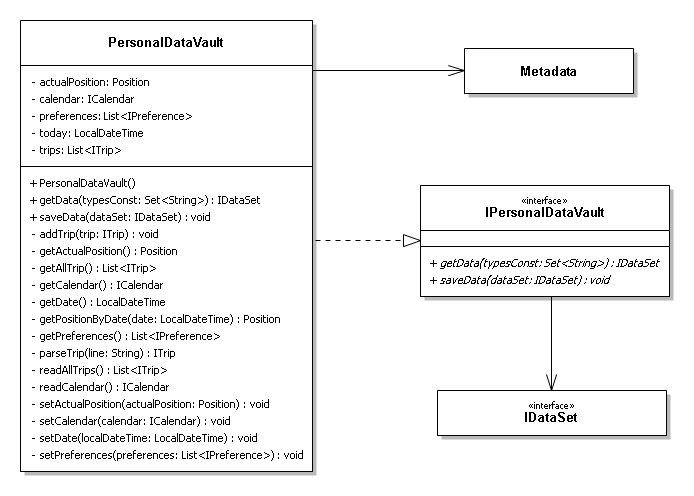
\includegraphics[width=0.8\linewidth]{pictures/PersonalDataVault.png}
	\caption{Diagramma UML dell'implementazione di un Personal Data Storage}
	\label{fig:PersonalDataVault}
\end{figure}
In questa sezione si presenta la classe \texttt{PersonalDataVault}, in cui vengono mantenuti i dati personali dell’utente. Essa corrisponde direttamente al Personal Data Storage proposto all’interno della documentazione \textit{MyData}.

L’interfaccia \texttt{IPersonalDataVault} espone i metodi \texttt{getData (Set<String> typesConst)} (che restituisce un \texttt{IDataSet}) e \texttt{saveData (IDataSet dataSet)} che permettono l’accesso ai dati. Essi si occupano di prelevare dati, o salvarli, in base a quanto specificato dal \texttt{Set<String>} contenente l’insieme dei tipi di dato. Inoltre, la signature garantisce l’indipendenza dai tipi di dato in ingresso o in uscita dal Vault grazie all’uso di oggetti di tipo \texttt{DataSet} incapsulati in opportune interfacce \texttt{IDataSet}. 

All’interno della classe \texttt{PersonalDataVault} troviamo alcuni metodi privati necessari per la gestione dei dati memorizzati (ad esempio la lettura e la scrittura su file, con opportune funzioni di utility necessarie per il parsing). Le scelte effettuate in questo senso derivano da una precedente implementazione e sono state adattate solo in minima parte per motivi di compatibilit\`a. Per quanto riguarda invece i metodi ereditati dall’interfaccia, si evidenzia l’eventualit\`a di una \texttt{RuntimeException} (\texttt{ClassCastException}): il verificarsi di questo evento non \`e auspicabile, ma rappresenta comunque uno stato del sistema previsto e voluto. Qualora infatti un oggetto dovesse rivelarsi di un tipo diverso rispetto a quello dichiarato all’interno del \texttt{dataSet} ricevuto in ingresso, \`e opportuno che il programma segnali questa grave inconsistenza, terminando la sua esecuzione. Incidentalmente, il verificarsi di una situazione di questo tipo implica la non osservanza delle politiche e dei protocolli di sicurezza, pertanto si ritiene motivato l’utilizzo di questa eccezione di basso livello.

Si può osservare che l’implementazione del \texttt{PersonalDataVault} è particolarmente dipendente dai tipi di dato utilizzati dal servizio \textit{Most Likely Next Trip} scelto come caso di studio. Tale caratteristica costituisce una limitazione del gestore di dati personali realizzato in questa tesi e trova un riscontro all’interno delle problematiche evidenziate all’interno della sezione \ref{sec:P-datinonnotiapriori}. Anche la scelta di memorizzare i dati acquisiti all’interno di file di testo, derivata da una precedente implementazione, si colloca all’interno di un orizzonte limitato: alcune proposte di aggiornamento sono state discusse in \ref{sec:A-PDS}, e saranno oggetto di ulteriore discussione all’interno del capitolo \ref{capitolo6}.

\subsection{Rappresentazione: Metadata}
\label{subsec:P-metadata}
\begin{figure} [h]
	\centering
	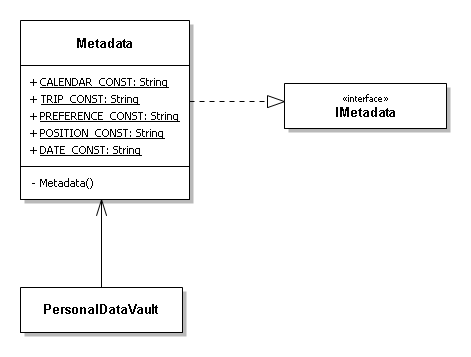
\includegraphics[width=0.7\linewidth]{pictures/Metadata.png}
	\caption{Diagramma UML della classe per la rappresentazione dei dati}
	\label{fig:Metadata}
\end{figure}
Come già accennato in precedenza, un approccio diverso, più completo ed esaustivo, avrebbe comportato mezzi più consistenti e conoscenze di cui - al momento - non si dispone.

Si è ritenuto, in alternativa, di dover ricorrere alla definizione preventiva dei tipi di dato disponibili all’interno del sistema, quali ad esempio \texttt{Position} e \texttt{ICalendar}, utilizzando dove possibile le interfacce al posto delle classi, onde diminuire la forte dipendenza dalla particolare implementazione.

Questa modalità potrebbe forse apparire come una eccessiva semplificazione del contesto per la scelta arbitraria dei tipi di alto livello sopra menzionati e delle loro implementazioni. La soluzione proposta, però, è da ritenersi plausibile in quanto valuta che i componenti indicati siano tali da poter rendere risultati accettabili anche in presenza delle limitazioni assunte.

Pertanto, la classe \texttt{Metadata} ha il compito di definire a priori i tipi di dato disponibili all’interno dell’Operatore \textit{MyData}. A livello implementativo, la classe espone un certo numero di stringhe \texttt{static final}, ognuna delle quali è inizializzata con il \textit{fully qualified name} della classe (o interfaccia) che rappresenta, al fine di conservare l’informazione completa riguardo al tipo di dato. All’interno del programma, esse sono accessibili mediante la notazione \texttt{Metadata.DATATYPE\_CONST}, ad esempio al momento della costruzione dei \texttt{Set<String>} necessari per la registrazione presso il \texttt{ServiceRegistry} (sottosezione \ref{subsec:P-serviceregistry}), o nel controllo della legittimità dell’emissione di un permesso (sottosezione \ref{subsec:P-CMConsStatus}).

\subsection{Trasferimento: IDataSet}
\begin{figure} [h]
	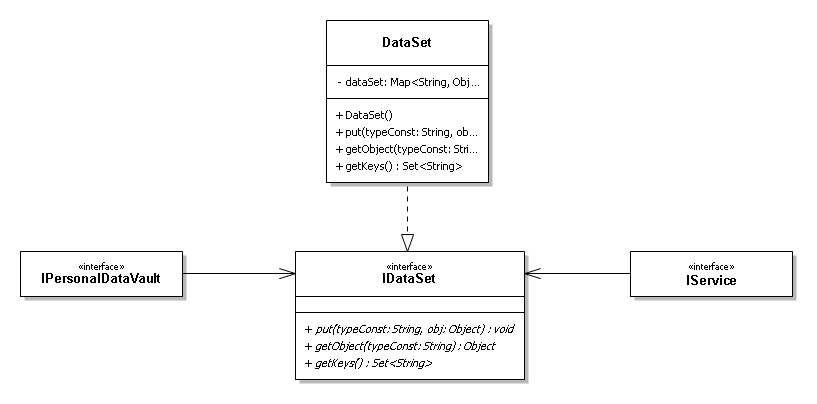
\includegraphics[width=\linewidth]{pictures/IDataSet.png}
	\caption{Diagramma UML della classe per il trasferimento dei dati}
	\label{fig:IDataSet}
\end{figure}
Come anticipato nelle sezioni precedenti, la classe \texttt{DataSet} viene utilizzata per il trasferimento di dati fra \textit{Source} e \textit{Sink}. Essa si riferisce e realizza il concetto di Resource Set Identifier, insieme alle oportune modifiche introdotte in fase di Analisi (sottosezione \ref{subsec:A-granularitaConsent}).
 Dal grafico UML in figura \ref{fig:IDataSet} si nota che essa viene sempre referenziata per mezzo dell’interfaccia \texttt{IDataSet}, ed è inoltre possibile riconoscere \texttt{IPersonalDataVault} e \texttt{IService} nei ruoli (non statici) di \textit{Source} e \textit{Sink}.

L’oggetto \texttt{DataSet} contiene i dati da trasferire mediante l’utilizzo di una \texttt{Map<String, Object>}, dove le chiavi sono le costanti di tipo stringa esposte dalla classe \texttt{Metadata} e i \textit{value} corrispondenti sono generici \texttt{Object} (non sono permessi valori \texttt{null}). In altre parole, questa struttura dati associa ad ogni oggetto il suo tipo, espresso all’interno di una stringa.

L’obiettivo della classe \texttt{DataSet} è contenere un insieme di oggetti potenzialmente diversi il cui tipo non è noto a priori, senza perdere l’informazione sul tipo stesso dopo la conversione a \texttt{Object}.

In questo modo si trova una soluzione al problema della \textit{Type Erasure}, poiché l’informazione sul tipo di dato originario viene conservata separatamente all’oggetto stesso. Il destinatario della trasmissione è in grado, attraverso le costanti di tipo stringa, di risalire al tipo dell’oggetto ricevuto, in modo da poterlo utilizzare in modo appropriato.

I metodi esposti dall’interfaccia ridefiniscono quelli propri della struttura dati \texttt{Map} che costituisce lo stato interno della classe, aggiungendo il controllo per i valori \texttt{null} e per la richiesta di oggetti non disponibili all’interno della mappa data.

\section{Uso delle eccezioni}
All’interno del gestore di dati personali sviluppato nell’ambito della tesi in oggetto, \`e di importanza non trascurabile il controllo della legittimit\`a delle operazioni da eseguire, degli argomenti in ingresso alle funzioni o degli stati in cui si trova il gestore stesso. Pertanto, \`e necessario uno strumento che permetta di descrivere il verificarsi di situazioni non previste o illegittime, impedendo la continuazione del flusso del programma. Questa situazione \`e diversa, ad esempio, dal caso in cui l’invocazione di un metodo \`e legittima ma non produce alcuni risultato, poich\'e \`e di fondamentale importanza che l’esecuzione termini.

Lo strumento utilizzato per ottenere questa caratteristica sono le Java \texttt{Exception}, ed in particolare le sottoclassi di \texttt{RuntimeException} \texttt{IllegalArgumentException}, \texttt{IllegalStateException} e \texttt{SecurityException}. 

Fra di esse, \texttt{IllegalStateException} \`e descritta all’interno della documentazione Java nel modo seguente: “Signals that a method has been invoked at an illegal or inappropriate time. In other words, the Java environment or Java application is not in an appropriate state for the requested operation” \cite{java8api}. Ho valutato quindi che questa eccezione fosse adeguata in tutti quei casi in cui l’invocazione di un metodo non pu\`o essere portata a termine a causa di Consent non adeguati. Un esempio pu\`o essere la richiesta di un nuovo \texttt{DataConsent} nel caso in cui non vi sia un \texttt{ServiceConsent} attivo in quel momento.

L’uso di \texttt{IllegalArgumentException} \`e convenzionalmente limitato al controllo dei parametri in ingresso ai metodi, in aderenza a quanto dichiarato sulla documentazione Java. Fra le \texttt{RuntimeException} utilizzate \`e presente anche \texttt{SecurityException}, invocata ogni volta in cui un parametro o controllo di sicurezza non \`e verificato.

Un aspetto importante dell’uso delle eccezioni \`e stata la loro collocazione all’interno dello \textit{stack} delle invocazioni di metodi. Si prenda di nuovo come esempio il caso di richiesta di un nuovo \texttt{DataConsent}: \`e noto a priori che la precondizione per ottenerlo richiede l’esistenza di un \texttt{ServiceConsent} attivo in quel momento. Questa eventualit\`a \`e controllata all’interno della classe \texttt{ConsentManager} mediante l’uso di una \texttt{IllegalStateException}. Tuttavia esiste un sotto-caso che, pur rientrando a pieno titolo nell’insieme di situazioni non corrette (mancanza di un \texttt{ServiceConsent} attivo) merita di essere differenziato per il suo valore semantico. Si tratta infatti del caso in cui l’utente per cui si sta facendo richiesta non sia registrato presso il servizio: il \texttt{ServiceConsent} non ha stato \textit{Active} perch\'e in realt\`a non ne \`e stato emesso alcuno. Al fine di controllare anche questa eventualit\`a \`e opportuno inserire una eccezione nella classe \texttt{MyDataUser} invece che \texttt{ConsentManager}, in quanto essa rientra all’interno del suo ambito di responsabilità.

\section{Graphical User Interface}
ddfd